\section{Obtained Results}

The results comprise the evaluation and implementation stages of CRISP-DM. In this section, we present the results obtained from the analysis of RAIS data. In general, the analyses comprise men and women in the IT sector in Brazil over the years.

In the graphs of the next subsections, pink lines were used to represent women and blue lines were used to represent men. The percentages displayed on women’s lines are relative to both salary differences and differences in the number of professionals and dismissals.

\subsection{Analysis with a data overview} \label{sub:geral}

\subsubsection{Quantity}

In Figure \ref{fig_1_qnt}, it is possible to verify that the quantity of men is greater than that of women. The greatest difference occurred in 2017, which was 74.85\%. In 2021, there was a small drop in this difference, which was 74.78\%

\begin{figure}[htbp]
	{
		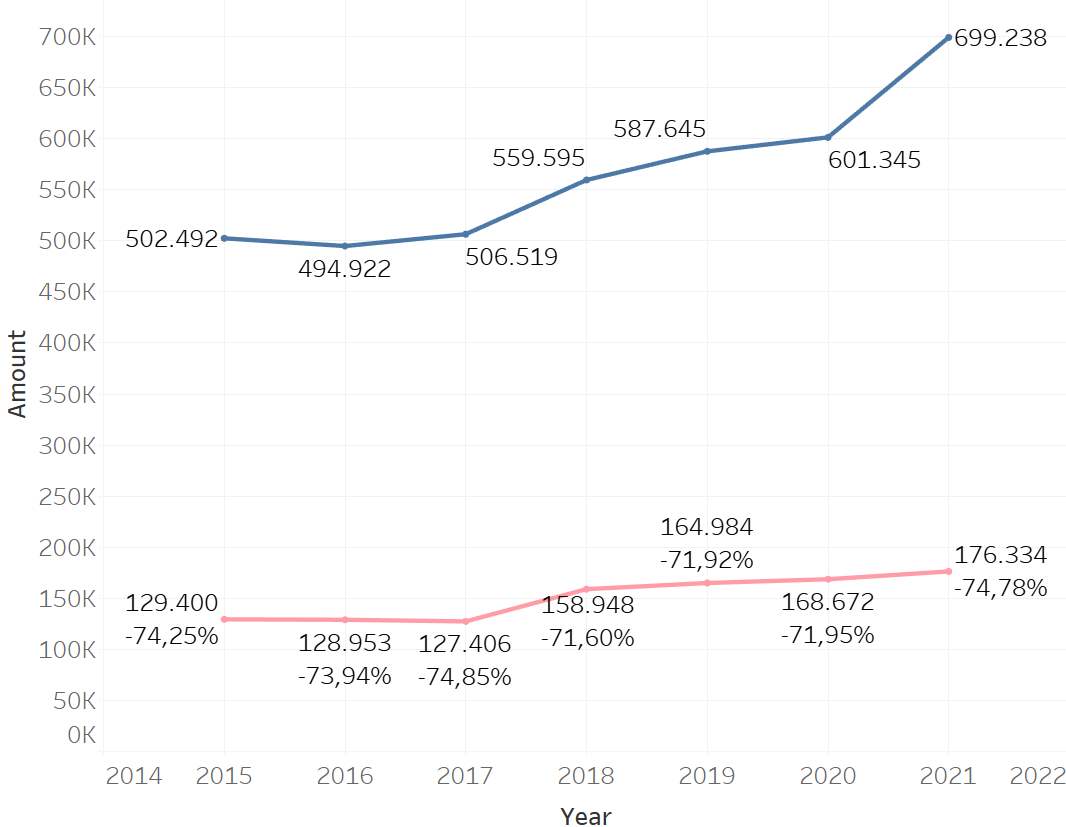
\includegraphics[width=85mm]{assets/1_qnt.PNG}
	}
	\caption{General Quantity}
	\label{fig_1_qnt}
\end{figure}

\subsubsection{Average salary}

In the graph of Figure \ref{fig_1_sal}, it is possible to verify that in all years the average salary of men is higher than that of women. This difference was smaller in 2015, which was 4.87\%. In 2021, this difference increased to 13.71\% and in 2021 it decreased again and was 11.56\%.

\begin{figure}[htbp]
	\centerline{
		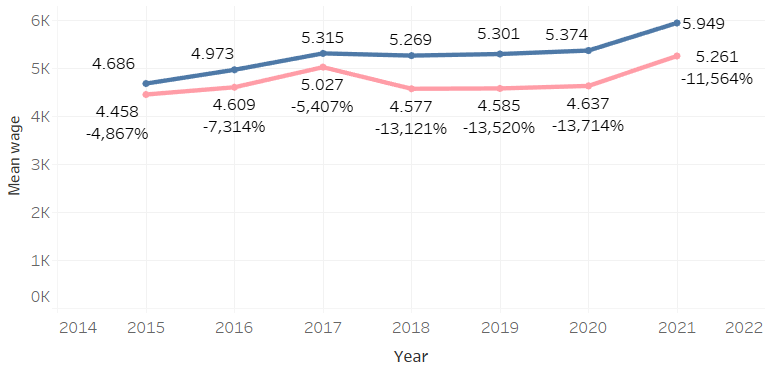
\includegraphics[width=85mm]{assets/1_sal.PNG}
	}
	\caption{Média salarial geral}
	\label{fig_1_sal}
\end{figure}


\subsection{Analysis by educational level}  \label{sub:educ}

\subsubsection{Quantity}

In Figure \ref{fig_2_qnt_educ}, it can be seen that for both genders there are more professionals with higher education compared to the number of professionals with only completed high school. The difference between the quantities of professionals by gender, both at the high school and higher education levels, varies between 71 and 78\%, being slightly higher at the high school level.

\begin{figure}[htbp]
	\centerline{
		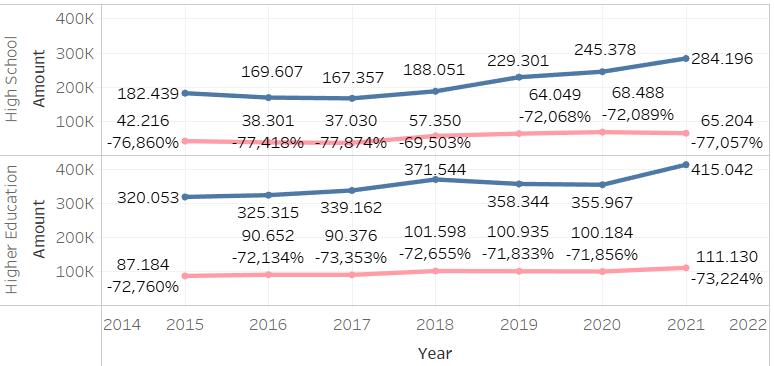
\includegraphics[width=85mm]{assets/2_qnt_educ.PNG}
	}
	\caption{Quantidade por nível educacional}
	\label{fig_2_qnt_educ}
\end{figure}

\subsubsection{Average salary}

For the average salary presented in Figure \ref{fig_2_sal_educ}, it is possible to verify that in all years the salary difference was higher at the high school level when compared to higher education. That is, women’s qualification seems to contribute to reducing wage inequality between genders in IT

\begin{figure}[htbp]
	\centerline{
		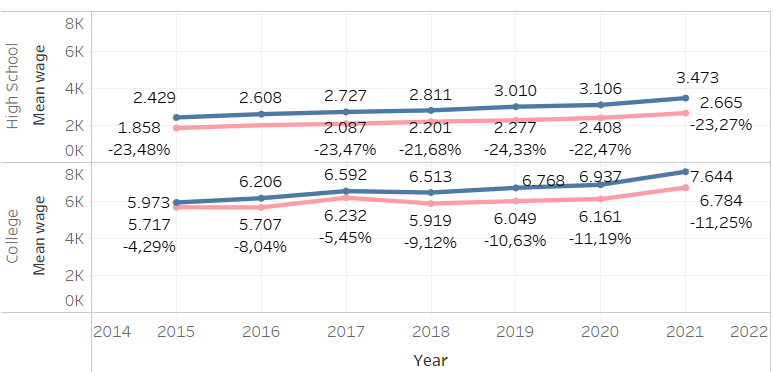
\includegraphics[width=85mm]{assets/2_sal_educ.PNG}
	}
	\caption{Média salarial por nível educacional}
	\label{fig_2_sal_educ}
\end{figure}

\subsection{Analysis by private and public sector}  \label{sub:privpub}

\subsubsection{Quantity}

In Figures \ref{fig_3_qnt_pubpriv} and \ref{fig_3_1_qnt_pubpriv}, it is possible to verify that the number of male professionals is higher than the number of female professionals, regardless of the sector. However, in the private sector the difference is even greater, as in the case of 2021, where this difference was 75.19\%, while in the public sector it was 61.09\%.

\begin{figure}[htbp]
	\centerline{
		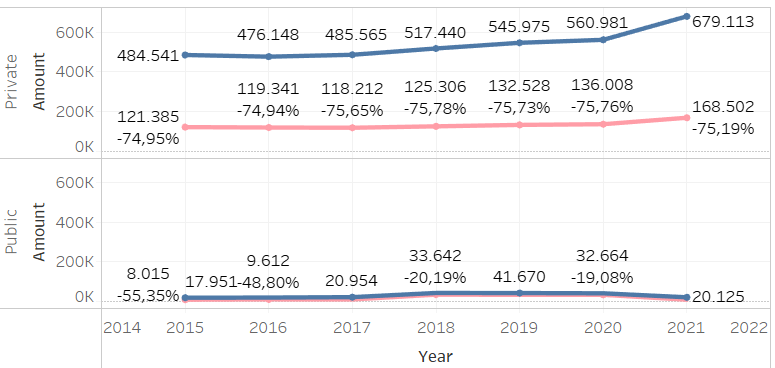
\includegraphics[width=85mm]{assets/3_qnt_pubpriv.PNG}
	}
	\caption{Quantity by sector}
	\label{fig_3_qnt_pubpriv}
\end{figure}


\begin{figure}[htbp]
	\centerline{
		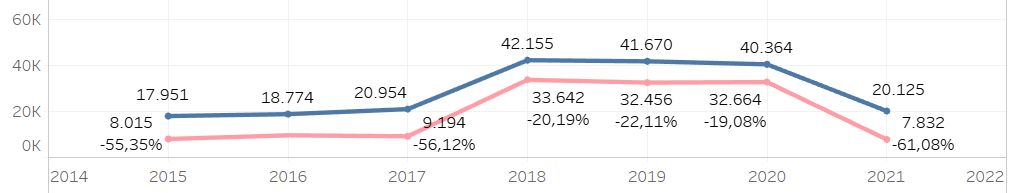
\includegraphics[width=85mm]{assets/3_1_qnt_pubpriv.PNG}
	}
	\caption{Extended quantity chart by public sector}
	\label{fig_3_1_qnt_pubpriv}
\end{figure}

\subsubsection{Average salary}

With regard to the average salaries presented in Figure \ref{fig_3_sal_pubpriv}, their percentage differences are similar when comparing the private sector with the overall picture of Figure \ref{fig_1_sal}. However, there is a much greater discrepancy in the percentage differences between 2018 and 2020 when looking at the public sector; the analyzed data does not allow for the identification of a possible cause for this phenomenon.

\begin{figure}[htbp]
	\centerline{
		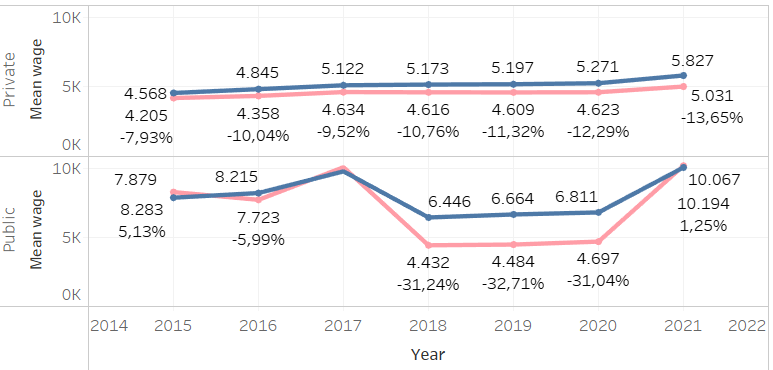
\includegraphics[width=85mm]{assets/3_sal_pubpriv.PNG}
	}
	\caption{Average salary by sector}
	\label{fig_3_sal_pubpriv}
\end{figure}

\subsection{Analysis of the amount of layoffs}

In this section, the analysis was carried out regarding the number of dismissals of male and female professionals. There is a chart for each gender. In each chart, the number of people dismissed is presented and, just below it, the number of people not dismissed, that is, kept in employment in the respective year. The percentage is also different because it analyzes the difference in relation to the previous data on its own line, not in relation to the other gender.

\subsubsection{Homem}

It is noteworthy, in Figure \ref{fig_4_qnt_h_demit}, that in 2021 the percentage of dismissal of male professionals was the highest in the last 7 years: 35.82\%. It is worth noting that 2021 was a critical year in relation to the COVID19 pandemic and that these dismissals may be related to the economic scenario of the time.

\begin{figure}[htbp]
	\centerline{
		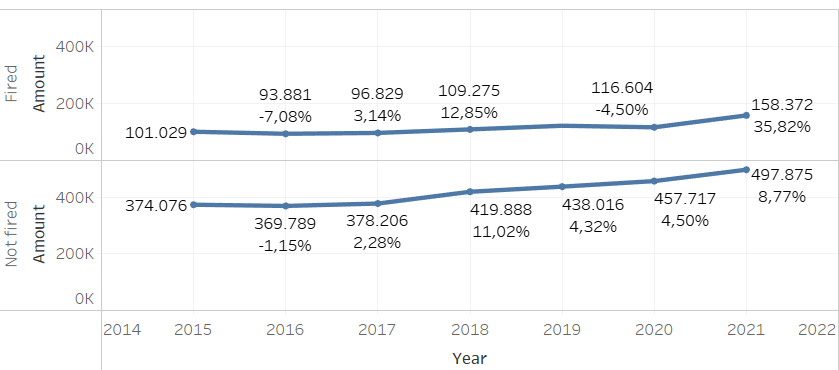
\includegraphics[width=85mm]{assets/4_qnt_h_demit.PNG}
	}
	\caption{Dismissals of men}
	\label{fig_4_qnt_h_demit}
\end{figure}

\subsubsection{Woman}

Similarly, in Figure \ref{fig_4_qnt_m_demit}, it is also possible to notice that in 2021 the percentage of dismissal of female professionals was the highest in the last 7 years: 29.91\%. This percentage is lower than that of men. Therefore, this is the only data where the asymmetry is favorable to women.

\begin{figure}[htbp]
	\centerline{
		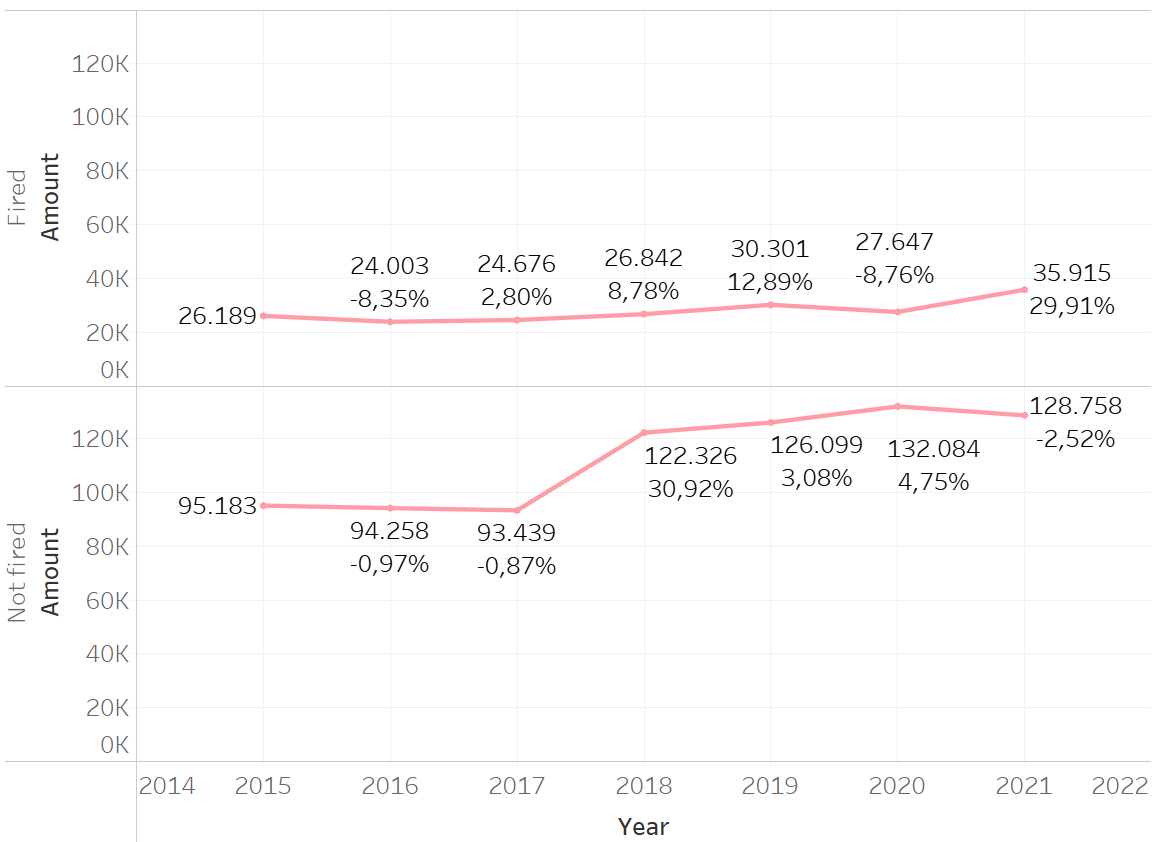
\includegraphics[width=85mm]{assets/4_qnt_m_demit.PNG}
	}
	\caption{Dismissals of women}
	\label{fig_4_qnt_m_demit}
\end{figure}

\subsection{Analysis by IT Job Title}

In the analyzes by positions, only the year 2021 was considered, as it is the last year available in our database and represents the most current data on the distribution of men and women among the various IT positions, both in the public and private sectors.

\subsubsection{Quantity}

According to Figure \ref{fig_5_qnt_cbo}, the position of Systems Development Analysts is the one that concentrates the largest number of IT professionals, both men and women, followed by Computer Support Analysts. In all professions, the number of men is greater than that of women, and the difference is greater in the position of Systems Development Analysts, where the number of men is almost 4 times greater than that of women.

\subsubsection{Average salary}

In Figure \ref{fig_5_sal_cbo}, it is possible to identify that the salary difference remains favorable for men, except for the position of Network and Data Communication Analyst, where the average salary of women is higher than that of men by 2.17\%. The largest salary difference in favor of men is related to the position of Computer Operator: 25.73\%, followed by Information Security Administrator: 19.75\% and Computer Engineer: 18.75\%. The lowest percentage differences are related to the positions of Information Systems Developer: 4.16\%, followed by Systems Development Analyst: 8.82\% and Internet Developer: 10\%. It can be concluded that the salary difference tends to be slightly lower in development areas in general.

\begin{figure}[htbp]
	\centerline{
		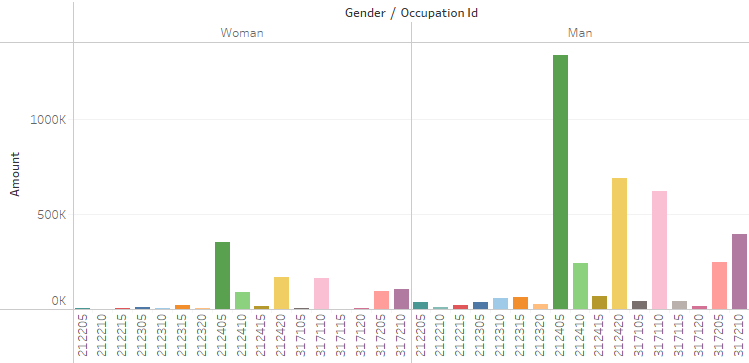
\includegraphics[width=85mm]{assets/5_qnt_cbo.PNG}
	}
	\caption{Quantity by Job in 2021}
	\label{fig_5_qnt_cbo}
\end{figure}

\begin{figure}[htbp]
	\centerline{
		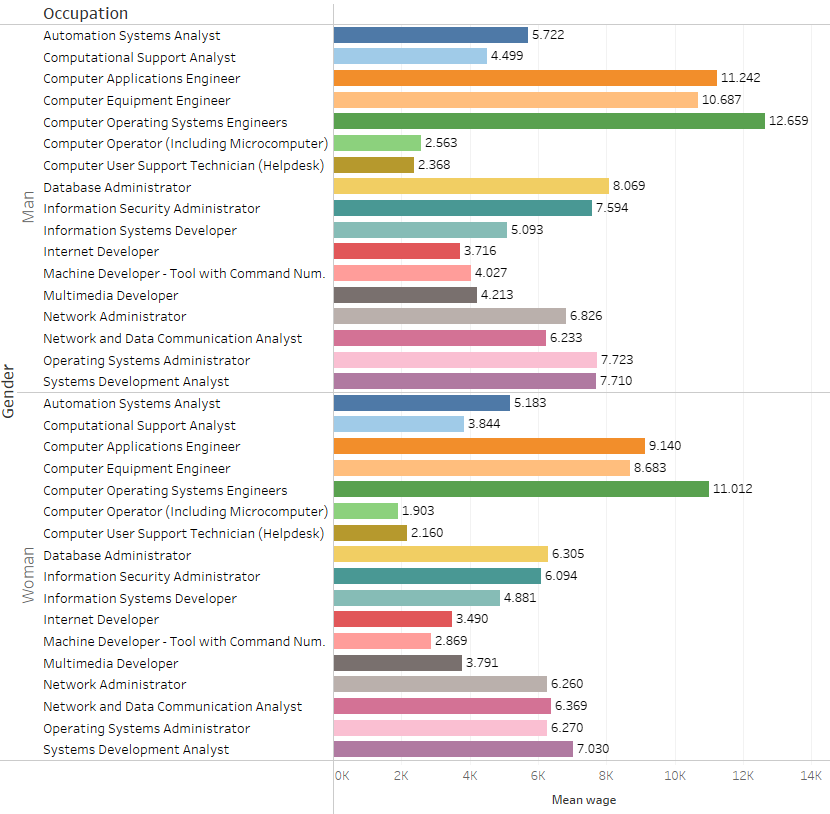
\includegraphics[width=85mm]{assets/5_sal_cbo.PNG}
	}
	\caption{Average salary per position in 2021}
	\label{fig_5_sal_cbo}
\end{figure}